\begin{figure}[h!]
	\centering
	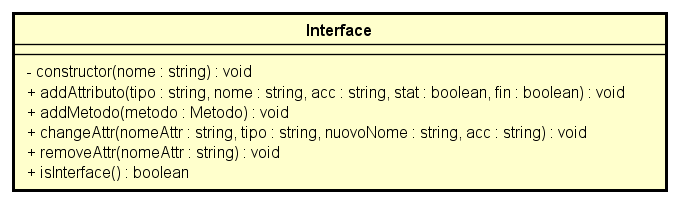
\includegraphics[scale=0.8]{res/sections/SpecificaFrontEnd/Services/Disegnetti/interface.png}
	\caption{Diagramma della classe Interface}
\end{figure}

\begin{itemize}
	item \textbf{Descrizione:}\\
	Modello che contiene tutti i metodi per la gestione dei campi dati di una Interfaccia.
	\item \textbf{Utilizzo:}\\
	Utilizzato per  la gestione dei campi dati di una Interfaccia.
	\item \textbf{Metodi:}
		\begin{itemize}
			\item \emph{-constructor(nome: string)}\\
    		Costruisce una nuova interfaccia\\
    		\textbf{Parametri:}
    		\begin{itemize}
    			\item \emph{nome: string}\\
    			Nome dell'interfaccia
    		\end{itemize}
    		\item \emph{+addAttributo(tipo: string, nome: string, acc: string, stat: boolean, fin: boolean)}\\
    		Aggiunge un attributo all'array di attributi dell'interfaccia\\
    		\textbf{Parametri:}
    		\begin{itemize}
    			\item \emph{tipo: string}\\
    			Tipo dell'attributo
    			\item \emph{nome: string}\\
    			Nome dell'attributo
    			\item \emph{acc: string}\\
    			Visibilità dell'attributo
    			\item \emph{stat: boolean}\\
    			True se è marcato static
    			\item \emph{fin: boolean}\\
    			True se è marcato final
    		\end{itemize}
    		\item \emph{+addMetodo(metodo: Metodo)}\\
    		Aggiunge un metodo all'array di metodi dell'interfaccia\\
    		\textbf{Parametri:}
    		\begin{itemize}
    			\item \emph{metodo: Metodo}\\
    			Netodo da aggiungere
    		\end{itemize}
    		\item \emph{+changeAttr(nomeAttr: string, tipo: string, nuovoNome: string, acc: string)}\\
    		Modifica un attributo dell'interfaccia\\
    		\textbf{Parametri:}
    		\begin{itemize}
    			\item \emph{nomeAttr: string}\\
    			Vecchio nome dell'attributo
    			\item \emph{tipo: string}\\
    			Tipo dell'attributo
    			\item \emph{nuovoNome: string}\\
    			Nuovo nome dell'attributo
    			\item \emph{acc: string}\\
    			Visibilità dell'attributo
    		\end{itemize}
    		\item \emph{+removeAttr(nomeAttr: string)}\\
    		Rimuove un attributo dalla lista degli attributi dell'interfaccia\\
    		\textbf{Parametri:}
    		\begin{itemize}
    			\item \emph{nomeAttr: string}\\
    			Nome dell'attributo da rimuovere
    		\end{itemize}
    		\item \emph{+isInterface()}\\
    		Ritorna true se è un interfaccia
    	\end{itemize}
\end{itemize}